\chapter{The Extraction Chart: Impedance, Reflection, and the Matching Problem}
\label{apx:extraction_chart}

The electrodynamic formalism developed in Chapter~\ref{ch:redefining} and consolidated in the
Equation Registry supplies a resistance $R$ (Equation~\ref{eq:19.8-systemic-resistance-registry}),
a capacitance $C$ (Equation~\ref{eq:19.9-enclosure-capacitance-registry}), an inductance $L$
(Equation~\ref{eq:19.10-inductive-kickback-registry}), a complex wage
$W = \psi_m + j\psi_s$ (Equation~\ref{eq:19.6-complex-wage-registry}), and a complex power
$S = P_{\text{real}} + jQ_{\text{reactive}}$ (Equation~\ref{eq:19.11-ac-complex-power-registry}).
These quantities are introduced separately and calibrated separately. This appendix supplies the
single geometric object on which all of them are simultaneously legible: the
\textbf{reflection-coefficient plane}, known in electrical engineering as the Smith chart and
called here the \textbf{Extraction Chart}.

The appendix also closes a definitional gap. Chapter~\ref{ch:spectral_carrier} reports a per-axis
impedance for the racial channel ($|Z| \approx 0.10$) and per-axis natural frequencies, and uses
those numbers to explain the observed $11{:}1$ resonance advantage. No reference impedance $Z_0$ is
defined anywhere in the manuscript, and no normalization is stated. Sections~\ref{sec:xc_normalization}
and~\ref{sec:xc_axes} supply both.

\medskip

\noindent\textbf{Confidence tier.} The formal apparatus of this appendix is Tier~3
(structural). It restates and unifies results already derived elsewhere in the book and introduces
no new calibrated measurement. The per-axis placements in Section~\ref{sec:xc_axes} inherit the
Tier~2 status of the spectral decomposition in Chapter~\ref{ch:spectral_carrier} for their
resistive components, and carry Tier~3 status for their reactive components, which depend on a
quality factor $Q_k$ that the present dataset does not resolve. Falsification criteria appear in
Section~\ref{sec:xc_falsification}.

\section{Port Convention}
\label{sec:xc_ports}

The manuscript describes power flowing in two directions. The Preface establishes that the kinetic
labor of $O_{\text{racialized}}$ and $I_{\text{buffer}}$ constitutes the actual power supply
$V_{cc}$, with $E$ operating as a gating control layer. Chapters~\ref{ch:tweedism}
and~\ref{ch:spectral_carrier} describe a suppression signal propagating downward from $E$ through
$P_{\text{uppet}}$ and $F_{\text{enforce}}$ into the lower tiers. A transmission-line treatment
requires these two directions to be fixed once and used consistently.

\begin{definition}[Extraction line convention]
The extraction architecture is modeled as a two-port network terminated in a load. The
\textbf{incident wave} $a$ is the suppression signal injected downward from $E$. The
\textbf{reflected wave} $b$ is the component returned upward as refusal, backlash, or
non-compliance. The \textbf{load} is the population upon which the suppression signal terminates.
Real power absorbed by the load is the power the population takes on and cannot return, and this
absorbed power is the extraction.
\end{definition}

This convention is a modeling choice rather than a derived result. It is adopted because it makes
the reflected wave $b$ the formal object corresponding to organized resistance, which is the
quantity the historical chapters track.

\section{Normalized Impedance and the Reflection Coefficient}
\label{sec:xc_normalization}

Let $Z_0$ denote the \textbf{characteristic impedance of the extraction line}: the impedance a
population presents when the suppression signal propagates through it without reflection. $Z_0$ is
set by the carrier established in Chapter~\ref{ch:spectral_carrier} and functions throughout as the
reference against which all other impedances are measured. Define the normalized impedance of a
load:

\begin{equation}\label{eq:xc.1-normalized-impedance}
z \;=\; \frac{Z}{Z_0} \;=\; r + jx
\end{equation}

The resistive component $r$ carries the material wage $\psi_m$ and performs real work. The reactive
component $x$ carries the psychological wage $\psi_s$ and performs no net work over a cycle. The
complex wage of Equation~\ref{eq:19.6-complex-wage-registry} is therefore an impedance, and
$W = \psi_m + j\psi_s$ is read as a position rather than a payment.

The reflection coefficient is the Möbius transform of the normalized impedance:

\begin{equation}\label{eq:xc.2-reflection-coefficient}
\Gamma \;=\; \frac{z - 1}{z + 1}, \qquad z \;=\; \frac{1 + \Gamma}{1 - \Gamma}
\end{equation}

Equation~\ref{eq:xc.2-reflection-coefficient} maps the entire right half-plane $\operatorname{Re}(z) \geq 0$
onto the closed unit disk $|\Gamma| \leq 1$. Every passive load in the system occupies a point in
that disk. The Extraction Chart is that disk.

The power absorbed by the load follows directly:

\begin{equation}\label{eq:xc.3-absorbed-power}
P_{\text{abs}} \;=\; |a|^2\bigl(1 - |\Gamma|^2\bigr)
\end{equation}

\noindent and the Reparations Integral (Equations~\ref{eq:0.16-reparations-integral}
and~\ref{eq:19.14-reparations-integral-registry}) admits an equivalent statement in wave variables:

\begin{equation}\label{eq:xc.4-reparations-wave-form}
\mathcal{R}(t_0, t_{\text{now}}) \;=\; \int_{t_0}^{t_{\text{now}}} \Bigl(|a(\tau)|^2 - |b(\tau)|^2\Bigr)\, d\tau
\end{equation}

Accumulated extraction is accumulated absorbed power: the portion of the incident suppression signal
that the population took on and did not return.

\subsection{The Enclosure Score as a Match Condition}

The Tri-Modal Enclosure Model (Equation~\ref{eq:1.1-enclosure-score}) measures the degree to which
an Out-group is denied all practical routes of escape, resilience, and structural self-perception,
with $\mathcal{S}_{\text{enc}} \to 1.0$ denoting absolute subjugation. A population with no route of
return reflects nothing:

\begin{equation}\label{eq:xc.5-enclosure-match}
\mathcal{S}_{\text{enc}} \;=\; 1 - |\Gamma|
\end{equation}

Total enclosure is a perfect impedance match. The center of the Extraction Chart, $\Gamma = 0$,
$z = 1$, $Z = Z_0$, is the condition the extraction algorithm optimizes toward. The rim,
$|\Gamma| = 1$, is withdrawn compliance: a purely reactive load that absorbs no real power. The
Preface states that the architecture dies when compliance is withdrawn.
Equation~\ref{eq:xc.3-absorbed-power} is the formal content of that statement.

The standing-wave ratio provides the system's diagnostic readout:

\begin{equation}\label{eq:xc.6-vswr}
\text{VSWR} \;=\; \frac{1 + |\Gamma|}{1 - |\Gamma|}
\end{equation}

Visible unrest is a standing-wave measurement. VSWR diverges as the load approaches the rim and
equals unity at perfect enclosure.

\section{The Buffer Class as a Lossless Matching Network}
\label{sec:xc_buffer}

The Buffer Work Theorem (Equation~\ref{eq:19.13-buffer-work-theorem-registry}) establishes that the
magnetic component of the extraction force performs zero net work on $I_{\text{buffer}}$:

\[
W_{I_{\text{buffer}}}^{\text{psych}}(t_0, t_1) = \int_{t_0}^{t_1} \mathbf{Q}\,(\vec{v} \times \vec{B}) \cdot \vec{v}\, d\tau \;\equiv\; 0
\]

Zero net work over a cycle with nonzero instantaneous magnitude is the defining property of a
reactive element. In network terms, an element that dissipates nothing, stores and returns energy
each cycle, and is inserted between a source and a load in order to eliminate reflection is a
\textbf{matching network}.

\begin{theorem}[Buffer Matching Theorem]
\label{thm:buffer-matching}
$I_{\text{buffer}}$ occupies the structural position of a lossless impedance-matching network
between $E$ and $O_{\text{racialized}}$. Its compensation is purely reactive: the time-averaged
real power delivered to $I_{\text{buffer}}$ is zero, while the reactive power $Q_{\text{reactive}}$
delivered to it is nonzero and sustained.
\end{theorem}

\begin{proof}[Argument]
By Equation~\ref{eq:19.13-buffer-work-theorem-registry} the psychological wage transfers no net
energy. By Equation~\ref{eq:19.11-ac-complex-power-registry} the complex power delivered to any
element decomposes as $S = P_{\text{real}} + jQ_{\text{reactive}}$, with $P_{\text{real}}$ the
time-averaged dissipation. An element with $P_{\text{real}} = 0$ and $Q_{\text{reactive}} \neq 0$ is
purely reactive. A purely reactive element placed in series or shunt between source and load
transforms the impedance the source sees without dissipating power, which is the definition of a
lossless matching network. The Buffer Class is positioned between $E$ and $O_{\text{racialized}}$
in the five-tier topology by construction (Chapter~\ref{ch:bacon}). \end{proof}

Theorem~\ref{thm:buffer-matching} resolves a question the historical chapters raise repeatedly and
answer only descriptively: why the Buffer Class defends a partition from which it accumulates
little. Reactive power has nonzero magnitude and zero time-average. The compensation is received in
full and is worth nothing at the end of each cycle. A matching network holds its position because
$|Q_{\text{reactive}}|$ is large, and it accumulates nothing because $P_{\text{real}}$ is zero.

On the chart, a lossless matching element moves a load along a constant-$r$ circle (series
reactance) or a constant-$g$ circle (shunt susceptance) without changing the real part. The
trajectory of $I_{\text{buffer}}$ across the historical record is a trajectory along such circles.

\section{Reform as Impedance Matching}
\label{sec:xc_reform}

Chapter~\ref{ch:contradiction} argues that reform serves the extraction algorithm. The chart
converts that argument into a monotonicity result.

\begin{theorem}[Reform Monotonicity]
\label{thm:reform-monotonicity}
Any intervention that strictly reduces $|\Gamma|$ strictly increases the real power absorbed by the
load. Formally, from Equation~\ref{eq:xc.3-absorbed-power},
\begin{equation}\label{eq:xc.7-reform-monotonicity}
\frac{\partial P_{\text{abs}}}{\partial |\Gamma|} \;=\; -2\,|a|^2\,|\Gamma| \;<\; 0
\qquad \text{for } |\Gamma| > 0
\end{equation}
\end{theorem}

Reforms that reduce friction, reduce backlash, and reduce refusal reduce $|\Gamma|$ by construction.
Reflection and extraction are the same variable carrying opposite signs, so an intervention cannot
reduce both. Reform operates as a matching stub.

The corollary specifies the direction of any anti-extractive intervention: increase $|\Gamma|$, move
outward on the chart toward the rim, and terminate in a purely reactive load. This is deliberate
mismatch, and it is the formal content of withdrawn compliance.

\section{Rotation, the Electoral Clock, and Quarter-Wave Co-optation}
\label{sec:xc_rotation}

On a lossless line, displacement of the reference plane rotates the reflection coefficient without
changing its magnitude:

\begin{equation}\label{eq:xc.8-rotation}
\Gamma(\ell) \;=\; \Gamma_L\, e^{-2j\beta \ell}, \qquad \beta = \frac{2\pi}{\lambda}
\end{equation}

One full rotation of the chart corresponds to $\ell = \lambda/2$. Chapter~\ref{ch:spectral_carrier}
establishes the four-year presidential cycle as the system's dominant spectral mode, with a
$24{:}1$ power advantage for identity-band language at $f = 0.25$~cyc/yr. Setting $\lambda$ equal to
the electoral cycle makes Equation~\ref{eq:xc.8-rotation} a clock.

\begin{theorem}[Quarter-Wave Co-optation]
\label{thm:quarter-wave}
Let a political formation present the extraction line with a short circuit, $z_L = 0$,
$\Gamma_L = -1$: total refusal, drawing the full suppression current and returning it inverted.
After a displacement of $\ell = \lambda/4$, the impedance presented at the new reference plane is
\begin{equation}\label{eq:xc.9-quarter-wave-transform}
z_{\text{in}} \;=\; \frac{1}{z_L} \;\longrightarrow\; \infty, \qquad \Gamma_{\text{in}} = +1
\end{equation}
which is an open circuit: a formation that draws no current and participates in nothing. The
composition of the load is unchanged throughout.
\end{theorem}

The transformation requires no change in the formation's membership, program, or intensity. Its
electrical distance from the generator changes, and the same load presents the system its exact
inverse. A further $\lambda/4$ returns it to a short. Militancy, irrelevance, and militancy recur
with a period fixed by the carrier rather than by the internal politics of the formation.

Theorem~\ref{thm:quarter-wave} yields a testable prediction: insurgent formations should exhibit
periodicity phase-locked to the electoral carrier, detectable by the same spectral method
Chapter~\ref{ch:spectral_carrier} applies to congressional language. The time-domain test that
failed in that chapter ($t = 0.479$, $p = 0.634$) failed for the reason stated there, namely that
phase-locked oscillations with variable amplitude are invisible to tests that ignore phase. The same
methodological point applies here.

\subsection{Attenuation and Manufactured Consent}

On a lossy line the reflection coefficient spirals inward toward the center with distance:

\begin{equation}\label{eq:xc.10-lossy-spiral}
\Gamma(\ell) \;=\; \Gamma_L\, e^{-2\alpha \ell}\, e^{-2j\beta \ell}
\end{equation}

An observer positioned at electrical distance $\ell$ from the load measures $|\Gamma|$ reduced by
$e^{-2\alpha\ell}$ and reads the system as matched. Attenuation manufactures the appearance of
consent. Historical distance from the site of extraction produces apparent settlement as an
artifact of the line, and the load itself is unchanged.

\section{Non-Reciprocity: The Enforcement Class as an Isolator}
\label{sec:xc_isolator}

The lethal-autonomy gradient (Equation~\ref{eq:6.1-lethal-autonomy-gradient}) states
\[
\text{Lethal Autonomy}(F_{\text{enforce}}) \gg \text{Lethal Autonomy}(I_{\text{buffer}}) \gg \text{Lethal Autonomy}(O) = 0
\]
In scattering parameters this is a statement about a two-port network:

\begin{equation}\label{eq:xc.11-nonreciprocity}
|S_{21}| \;\gg\; |S_{12}| \;\approx\; 0
\end{equation}

Force passes downward through $F_{\text{enforce}}$ and does not pass back up. A device with this
property is an \textbf{isolator}.

Lorentz reciprocity holds for any linear medium whose permittivity and permeability tensors are
symmetric, and it forces $S_{12} = S_{21}$. Violating reciprocity requires nonlinearity,
time-variance, or a static magnetic bias that renders the permeability tensor antisymmetric. The
standard engineering realization is a ferrite held in an applied DC magnetic field. The bias field
performs no work on the signal and is the sole reason the device conducts in one direction.

\begin{theorem}[Cultural Bias and Non-Reciprocity]
\label{thm:cultural-bias}
The cultural magnetic field $\vec{B}$ defined in Section~\ref{sec:trimodal} functions as the static
bias that breaks reciprocity in the enforcement tier. Removing the bias restores $S_{12} = S_{21}$,
under which force applied downward can propagate upward with equal transmission.
\end{theorem}

Theorem~\ref{thm:cultural-bias} supplies the load-bearing role of a field that performs no work. The
framework establishes in Equation~\ref{eq:19.13-buffer-work-theorem-registry} that $\vec{B}$
transfers no energy, and the Tri-Modal Enclosure Model assigns the psychological mode $e_3$ to it.
The isolator identification explains why a channel that transfers zero energy is structurally
indispensable: the asymmetry of the enforcement tier exists only under magnetic bias, and the
enforcement tier becomes a symmetric two-way channel without it.

\section{The Active Region and the Counter-Virus}
\label{sec:xc_active}

Every passive load satisfies $\operatorname{Re}(z) \geq 0$ and therefore $|\Gamma| \leq 1$. The
condition

\begin{equation}\label{eq:xc.12-active-condition}
|\Gamma| > 1 \quad \Longleftrightarrow \quad \operatorname{Re}(z) < 0
\end{equation}

requires negative resistance: an element that returns more power than it receives.
Equation~\ref{eq:xc.12-active-condition} is also the oscillation condition. A network terminated in
a negative resistance does not settle to a steady state and instead grows without bound at the
frequency where the loop gain exceeds unity.

Chapter~\ref{ch:algorithmic_epoch} calls for a counter-virus. Equation~\ref{eq:xc.12-active-condition}
defines it. Every point inside the unit disk is a passive load absorbing some fraction of the
incident suppression signal, and repositioning within the disk changes that fraction. Leaving the
disk requires the population to function as a source. This is consistent with the resonance result
of Chapter~\ref{ch:lagrangian}, where sustained coordination at the natural frequency
$\omega_0 = 1/\sqrt{LC}$ drives the response of a low-resistance system without bound.

The compactification is itself a result. Equation~\ref{eq:xc.2-reflection-coefficient} maps an
infinite half-plane onto a bounded disk with a fixed boundary. Appendix~\ref{app:universality}
conjectures that the topology of power is finite. The Extraction Chart is the statement that
unlimited variation in impedance occupies a bounded space with a fixed edge.

\section{The Bode--Fano Limit on Simultaneous Axes}
\label{sec:xc_bodefano}

The chart is defined at a single frequency. The framework is explicitly multi-band:
Chapter~\ref{ch:spectral_carrier} resolves race, gender, and sexuality into sub-bands with distinct
natural frequencies. Matching a reactive load across a bandwidth rather than at a point is bounded
by the Bode--Fano criterion. For a load reducible to a parallel $RC$ combination,

\begin{equation}\label{eq:xc.13-bode-fano}
\int_{0}^{\infty} \ln\frac{1}{|\Gamma(\omega)|}\, d\omega \;\leq\; \frac{\pi}{RC}
\end{equation}

The integral is a fixed budget. Improving the match over one band requires accepting a worse match
over another. Equation~\ref{eq:xc.13-bode-fano} is a quantitative statement of the cannibalization
argument in Chapter~\ref{ch:full_algo}: the system cannot hold every axis matched at once, and
tightening enclosure on one axis necessarily loosens it elsewhere in the spectrum. The historical
pattern of sequential axis activation follows from a conserved matching budget.

\section{Per-Axis Placement}
\label{sec:xc_axes}

Chapter~\ref{ch:spectral_carrier} reports natural frequencies for the three identity sub-bands: race
at $3.6$~yr, gender at approximately $6$~yr, and sexuality threshold-activated after 2003. Modeling
each axis as a series resonant branch driven at the four-year carrier, the normalized branch
impedance is

\begin{equation}\label{eq:xc.14-branch-impedance}
z_k(\omega) \;=\; r_k\Bigl[1 + jQ_k\,\delta_k\Bigr], \qquad
\delta_k \;=\; \frac{\omega}{\omega_{0,k}} - \frac{\omega_{0,k}}{\omega}
\end{equation}

The detuning $\delta_k$ follows directly from the published periods and requires no additional
assumption:

\begin{center}
\begin{tabular}{lccc}
\toprule
Axis & Natural period & $\omega/\omega_{0,k}$ & $\delta_k$ \\
\midrule
Race       & $3.6$~yr & $0.900$ & $-0.211$ \\
Gender     & $6.0$~yr & $1.500$ & $+0.833$ \\
Sexuality  & threshold-activated & --- & small, positive \\
\bottomrule
\end{tabular}
\end{center}

The sign of $\delta_k$ is the robust result. Race is driven below its natural frequency and presents
a capacitive reactance, placing it below the real axis. Gender is driven above its natural frequency
and presents an inductive reactance, placing it well above the real axis and far from match. The
magnitude of each reactance requires the quality factor $Q_k$, which the present dataset does not
resolve; the placements in Figure~\ref{fig:extraction_chart} use $Q_k = 3$ as an illustrative
normalization and are Tier~3 in their reactive component.

\subsection{Phase Loading as Current Division}

The identification of the axes as parallel branches supplies a circuit-theoretic definition for the
phase-loading coefficients $\rho_k$ that appear in the Spectral Carrier
(Equation~\ref{eq:19.12-n-weighted-phase-registry}), the Unified Lorentz Force
(Equation~\ref{eq:19.5-unified-lorentz-force-registry}), and the Reparations Integral
(Equation~\ref{eq:0.16-reparations-integral}):

\begin{equation}\label{eq:xc.15-phase-loading-current-division}
\rho_k \;=\; \frac{Y_k}{\sum_{i=1}^{N} Y_i}, \qquad Y_k = \frac{1}{Z_k}
\end{equation}

The suppression current divides among the available axes in proportion to branch admittance. The
axis with the lowest impedance carries the largest share. Race carries $|Z| \approx 0.10$, the
lowest of the three, and receives the largest $\rho_k$, which is the same claim as the $11{:}1$
resonance advantage expressed as a current-division ratio. Equation~\ref{eq:xc.15-phase-loading-current-division}
converts $\rho_k$ from an assigned weight into a derived quantity.

\begin{figure}[htbp]
\centering
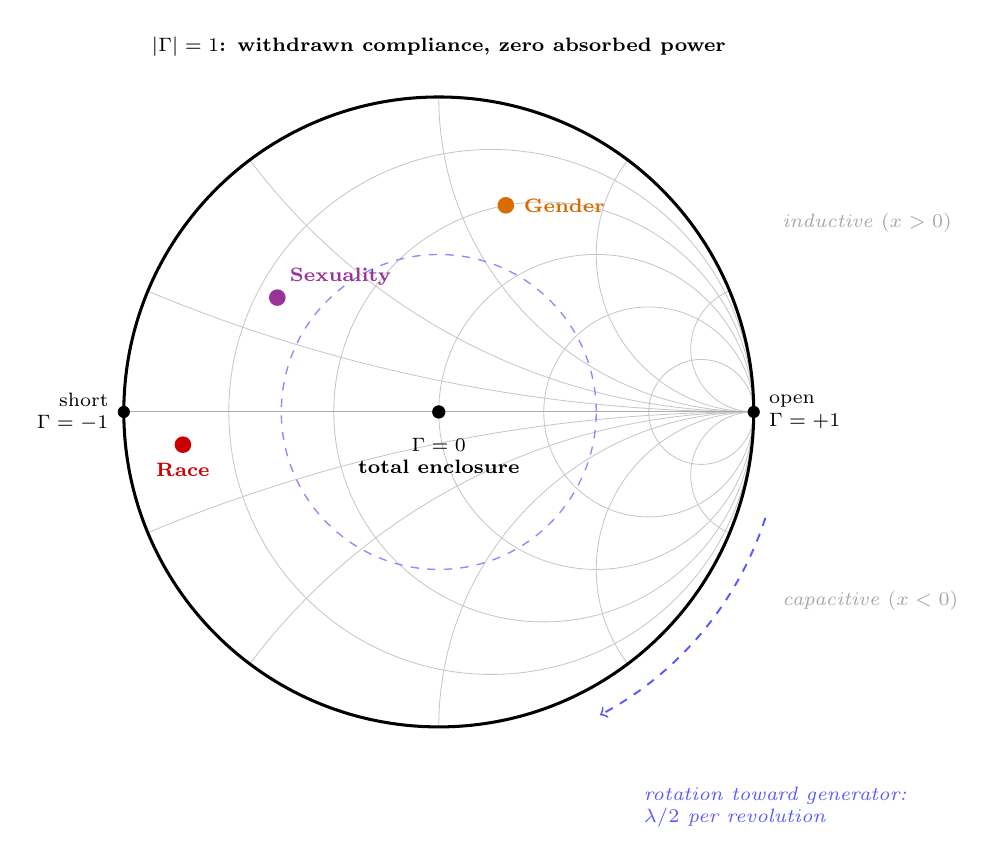
\begin{tikzpicture}[scale=1.0]
  \def\Rad{4}

  % --- clip everything to the unit disk ---
  \begin{scope}
    \clip (0,0) circle (\Rad);

    % constant-r circles: center (R*r/(1+r), 0), radius R/(1+r)
    \foreach \r in {0.2, 0.5, 1, 2, 5} {
      \pgfmathsetmacro{\cx}{\Rad*\r/(1+\r)}
      \pgfmathsetmacro{\rr}{\Rad/(1+\r)}
      \draw[gray!45, line width=0.3pt] (\cx,0) circle (\rr);
    }

    % constant-x arcs: center (R, R/x), radius R/|x|
    \foreach \x in {0.2, 0.5, 1, 2, 5} {
      \pgfmathsetmacro{\cy}{\Rad/\x}
      \pgfmathsetmacro{\rr}{\Rad/\x}
      \draw[gray!45, line width=0.3pt] (\Rad,\cy) circle (\rr);
      \draw[gray!45, line width=0.3pt] (\Rad,-\cy) circle (\rr);
    }

    % real axis
    \draw[gray!65, line width=0.4pt] (-\Rad,0) -- (\Rad,0);

    % constant-|Gamma| reference circle at 0.5
    \draw[blue!45, dashed, line width=0.5pt] (0,0) circle (0.5*\Rad);
  \end{scope}

  % --- unit circle: withdrawn compliance ---
  \draw[black, line width=1.1pt] (0,0) circle (\Rad);

  % --- terminal points ---
  \fill[black] (0,0) circle (2.4pt);
  \node[below=3pt, font=\scriptsize\bfseries, align=center] at (0,-0.1)
    {$\Gamma=0$\\ total enclosure};

  \fill[black] (-\Rad,0) circle (2.2pt);
  \node[left=2pt, font=\scriptsize, align=right] at (-\Rad,0)
    {short\\ $\Gamma=-1$};

  \fill[black] (\Rad,0) circle (2.2pt);
  \node[right=2pt, font=\scriptsize, align=left] at (\Rad,0)
    {open\\ $\Gamma=+1$};

  % --- region labels (placed outside the disk to avoid the plotted axes) ---
  \node[font=\scriptsize\itshape, gray!70, anchor=west] at (1.06*\Rad, 0.60*\Rad) {inductive $(x>0)$};
  \node[font=\scriptsize\itshape, gray!70, anchor=west] at (1.06*\Rad,-0.60*\Rad) {capacitive $(x<0)$};
  \node[font=\scriptsize\bfseries, align=center] at (0, 1.16*\Rad)
    {$|\Gamma| = 1$: withdrawn compliance, zero absorbed power};

  % --- measured axis placements (Q_k = 3 illustrative) ---
  % Race: z = 0.10 - j0.063  ->  Gamma = (-0.812, -0.104)
  \fill[red!80!black] (-3.249,-0.416) circle (3pt);
  \node[font=\scriptsize\bfseries, red!80!black, below=3pt] at (-3.249,-0.416) {Race};

  % Gender: z = 0.50 + j1.25  ->  Gamma = (0.213, 0.656)
  \fill[orange!85!black] (0.852,2.624) circle (3pt);
  \node[font=\scriptsize\bfseries, orange!85!black, right=3pt] at (0.852,2.624) {Gender};

  % Sexuality: z = 0.25 + j0.30  ->  Gamma = (-0.513, 0.363)
  \fill[violet!80] (-2.050,1.452) circle (3pt);
  \node[font=\scriptsize\bfseries, violet!80, above right=1pt] at (-2.050,1.452) {Sexuality};

  % --- quarter-wave rotation arc, drawn outside the disk ---
  \draw[->, blue!65, line width=0.7pt, dashed]
    (4.147,-1.347) arc[start angle=-18, end angle=-62, radius=4.36];
  \node[font=\scriptsize\itshape, blue!65, align=left, anchor=north west]
    at (0.62*\Rad, -1.16*\Rad)
    {rotation toward generator:\\ $\lambda/2$ per revolution};

\end{tikzpicture}
\caption[The Extraction Chart]{\textbf{The Extraction Chart.} The reflection-coefficient plane of
the extraction line. Every passive load occupies a point in the unit disk. The center
($\Gamma = 0$, $z = 1$) is a perfect impedance match and corresponds to total enclosure,
$\mathcal{S}_{\text{enc}} \to 1.0$, with all incident suppression absorbed and nothing returned. The
rim ($|\Gamma| = 1$) is withdrawn compliance: a purely reactive termination absorbing zero real
power. Grey circles are loci of constant normalized resistance $r$ (material wage) and constant
normalized reactance $x$ (psychological wage). Displacement along the line rotates a load clockwise
about the center at one revolution per $\lambda/2$, which places a short circuit at the open-circuit
point after $\lambda/4$ (Theorem~\ref{thm:quarter-wave}). Coloured markers place the three identity
sub-bands of Chapter~\ref{ch:spectral_carrier} using their published natural frequencies via
Equation~\ref{eq:xc.14-branch-impedance}; the sign of each reactance follows from the reported
periods, and the magnitudes assume $Q_k = 3$ as an illustrative normalization (Tier~3).}
\label{fig:extraction_chart}
\end{figure}

\section{Falsification Criteria}
\label{sec:xc_falsification}

The claims of this appendix fail under the following conditions.

\begin{enumerate}
    \item \textbf{Buffer Matching Theorem.} A longitudinal dataset showing that $I_{\text{buffer}}$
    accumulates real material wealth attributable to the psychological wage, net of its own labor
    contribution, over a period exceeding one generation. Nonzero time-averaged $P_{\text{real}}$
    delivered to the Buffer Class falsifies Theorem~\ref{thm:buffer-matching}.

    \item \textbf{Reform Monotonicity.} A documented intervention that measurably reduced backlash,
    refusal, and non-compliance while simultaneously reducing the extraction rate
    $d\mathcal{E}/dt$. Equation~\ref{eq:xc.7-reform-monotonicity} forbids this pairing.

    \item \textbf{Quarter-Wave Co-optation.} Spectral analysis of insurgent-formation activity
    showing no power concentration at the electoral carrier or its harmonics across a dataset of
    comparable length to the 60-year congressional series. Absence of phase-locking falsifies
    Theorem~\ref{thm:quarter-wave}.

    \item \textbf{Cultural Bias and Non-Reciprocity.} A documented enforcement architecture
    exhibiting the lethal-autonomy gradient of
    Equation~\ref{eq:6.1-lethal-autonomy-gradient} in the absence of any cultural or
    psychological partition. Sustained non-reciprocity without bias falsifies
    Theorem~\ref{thm:cultural-bias}.

    \item \textbf{Bode--Fano Limit.} A historical period in which enclosure tightened simultaneously
    and durably across all identity axes without compensating loosening on any axis.
    Equation~\ref{eq:xc.13-bode-fano} forbids an unbounded matching budget.

    \item \textbf{Phase loading as current division.} Measured $\rho_k$ values departing from the
    admittance ratio of Equation~\ref{eq:xc.15-phase-loading-current-division} beyond the
    uncertainty of the per-axis impedance estimates.
\end{enumerate}

\section{Open Problems}
\label{sec:xc_open}

Three quantities in this appendix are asserted rather than measured, and each is resolvable with
existing data.

$Z_0$ is defined structurally in Section~\ref{sec:xc_normalization} and is not fitted. Estimating it
from the congressional-record spectral series would place the per-axis impedances on an absolute
scale and upgrade the placements in Figure~\ref{fig:extraction_chart} from Tier~3 to Tier~2.

The quality factors $Q_k$ control the reactive magnitudes and are currently set to an illustrative
constant. Resolving them requires higher-frequency data than the annual series supports, which is
the same resolution limit that left the two-year midterm cycle indeterminate in
Chapter~\ref{ch:spectral_carrier}.

The Bode--Fano budget in Equation~\ref{eq:xc.13-bode-fano} has not been evaluated numerically. A
computed bound would convert the cannibalization argument from an ordinal claim into a stated
maximum on the number of axes the architecture can hold matched at once.
